This chapter will present the actual implementation of our model in the \textit{Simulink} environment together with the open-loop analysis of stability.

\section{Implementation}
\subsection{Motors}
The model of the motors is displayed in Figure \ref{motorr}. Each transfer function was obtaineed by putting the coefficients obtained in Section x in place. The deadzone for each motor was also added to the simulation. The output of the system is represented by the angular velocities of the propellers. 

\begin{figure}[H]
  \centering
    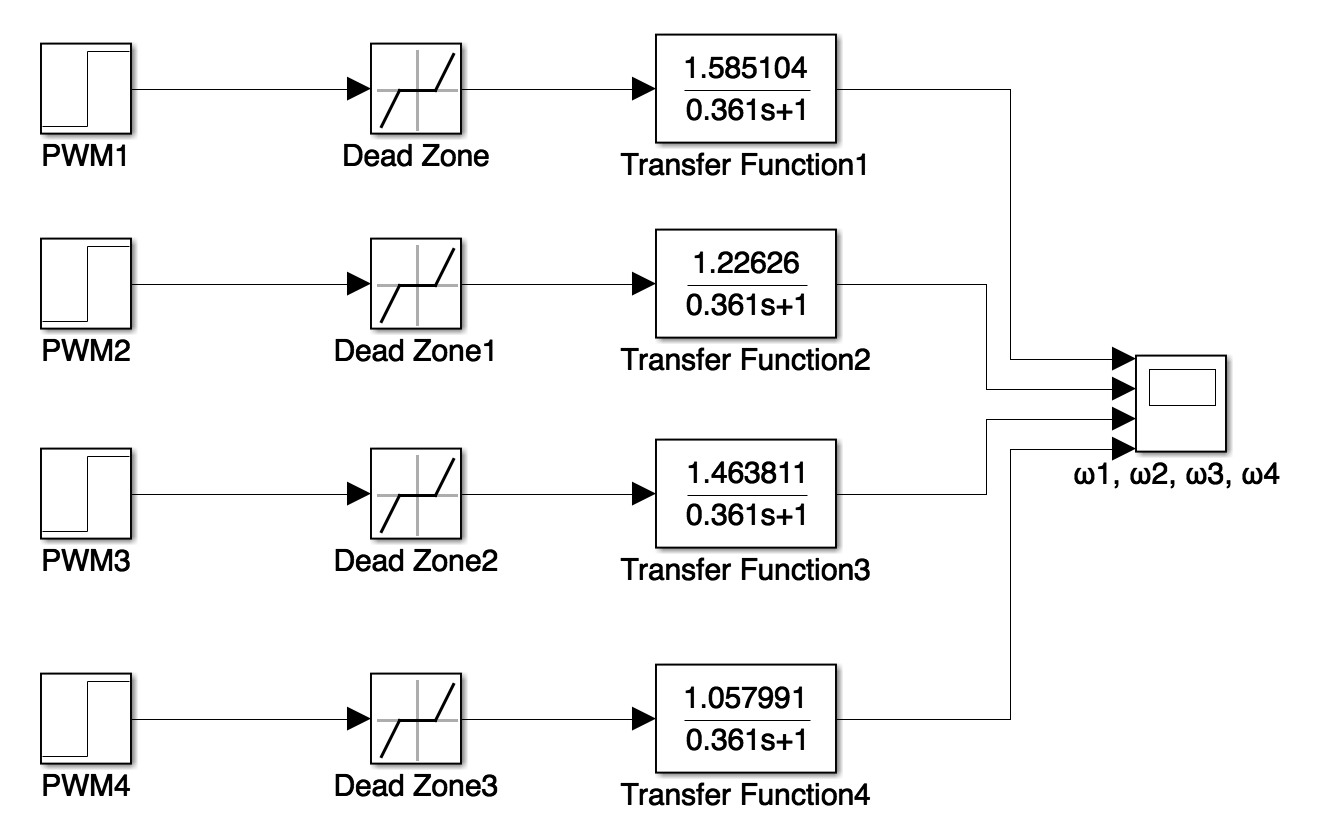
\includegraphics[width=0.9\textwidth]{images/simulinkmotor.png}
	\caption{Implementation of the motors' model.}
	\label{motorr}
\end{figure}

By giving the PWM values from Table \ref{motorCoeffs}, the simulation shows angular velocity of all four motors. It can be seen in Figure \ref{motorScope} that the speeds still do not match perfectly. This is because none of the functions are linear, giving only the approximations of the coefficients used in the model and not exact values. As such, some controller will need to be implemented to try and compensate for the differences.

\begin{figure}[H]
  \centering
    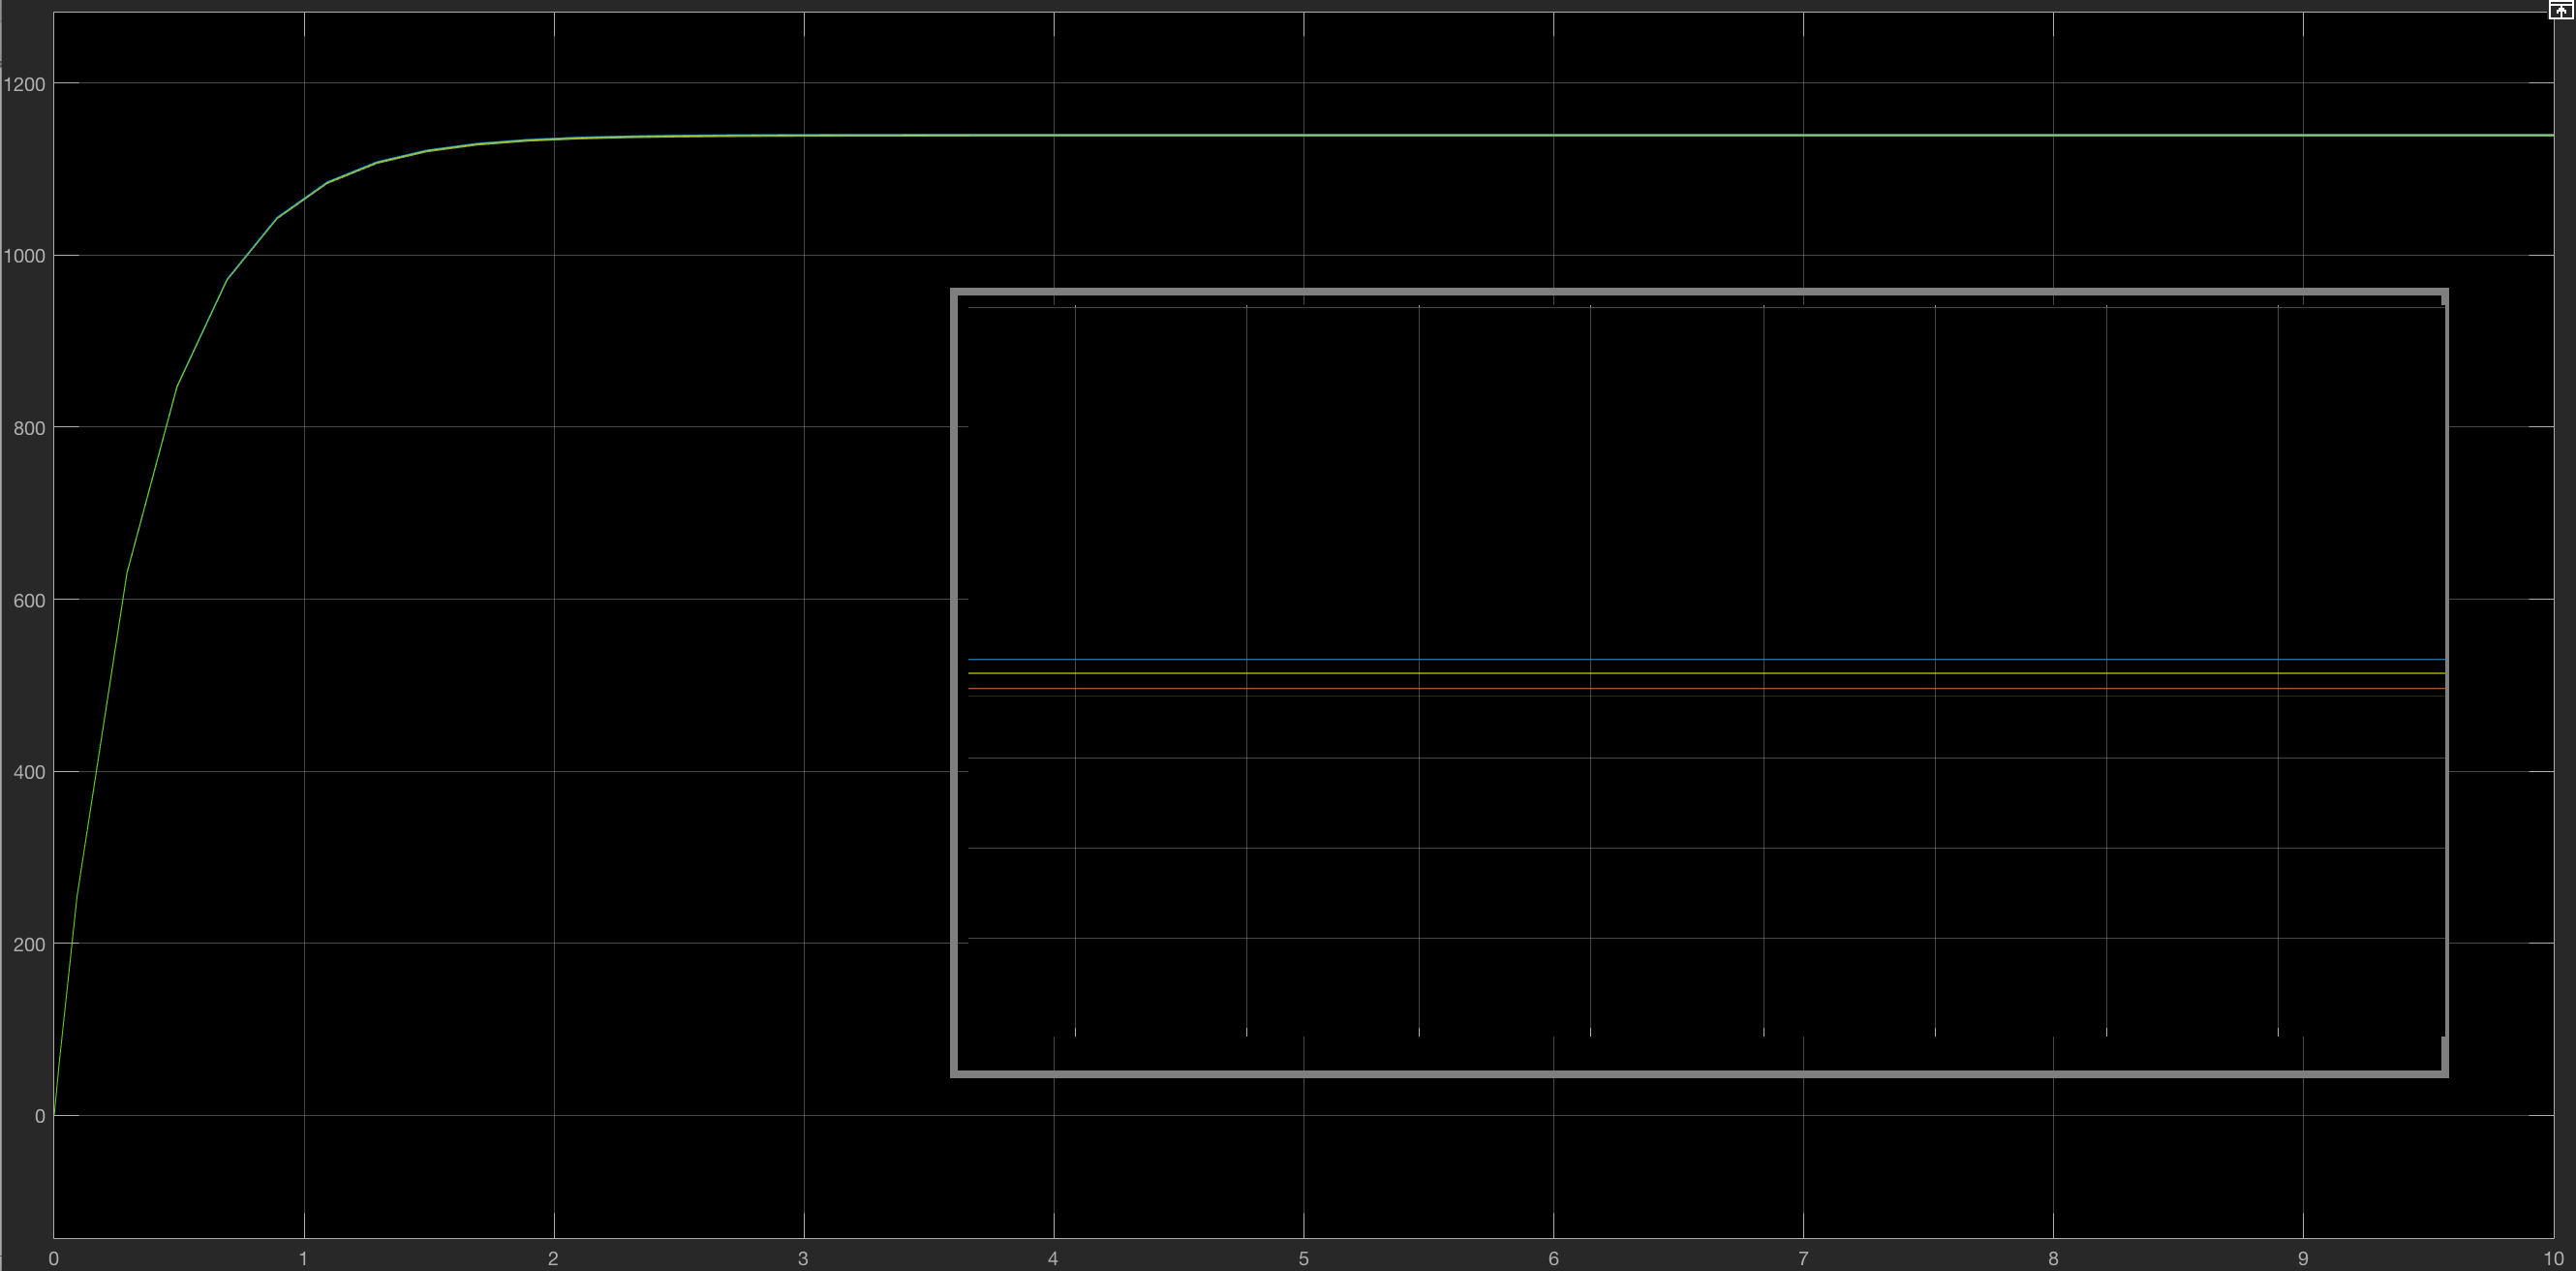
\includegraphics[width=1\textwidth]{images/scopewithcloseup.png}
	\caption{The Output of the Model and a Close Up.}
	\label{motorScope}
\end{figure}

\subsection{Model Simulation}
In order to make a complete model and simulate it, we have taken the model for the motors, which outputs the angular velocities $\omega_{1}, \omega_{2}, \omega_{3}, \omega_{4}$ and further extended it based on Equations \ref{motor1} - \ref{motor4}. The plant block contains the state space equations of the model and the scopes are represented by the the system's outputs. Figure \ref{openloop} illustrates the open loop Simulink model.

\begin{figure}[H]
  \centering
    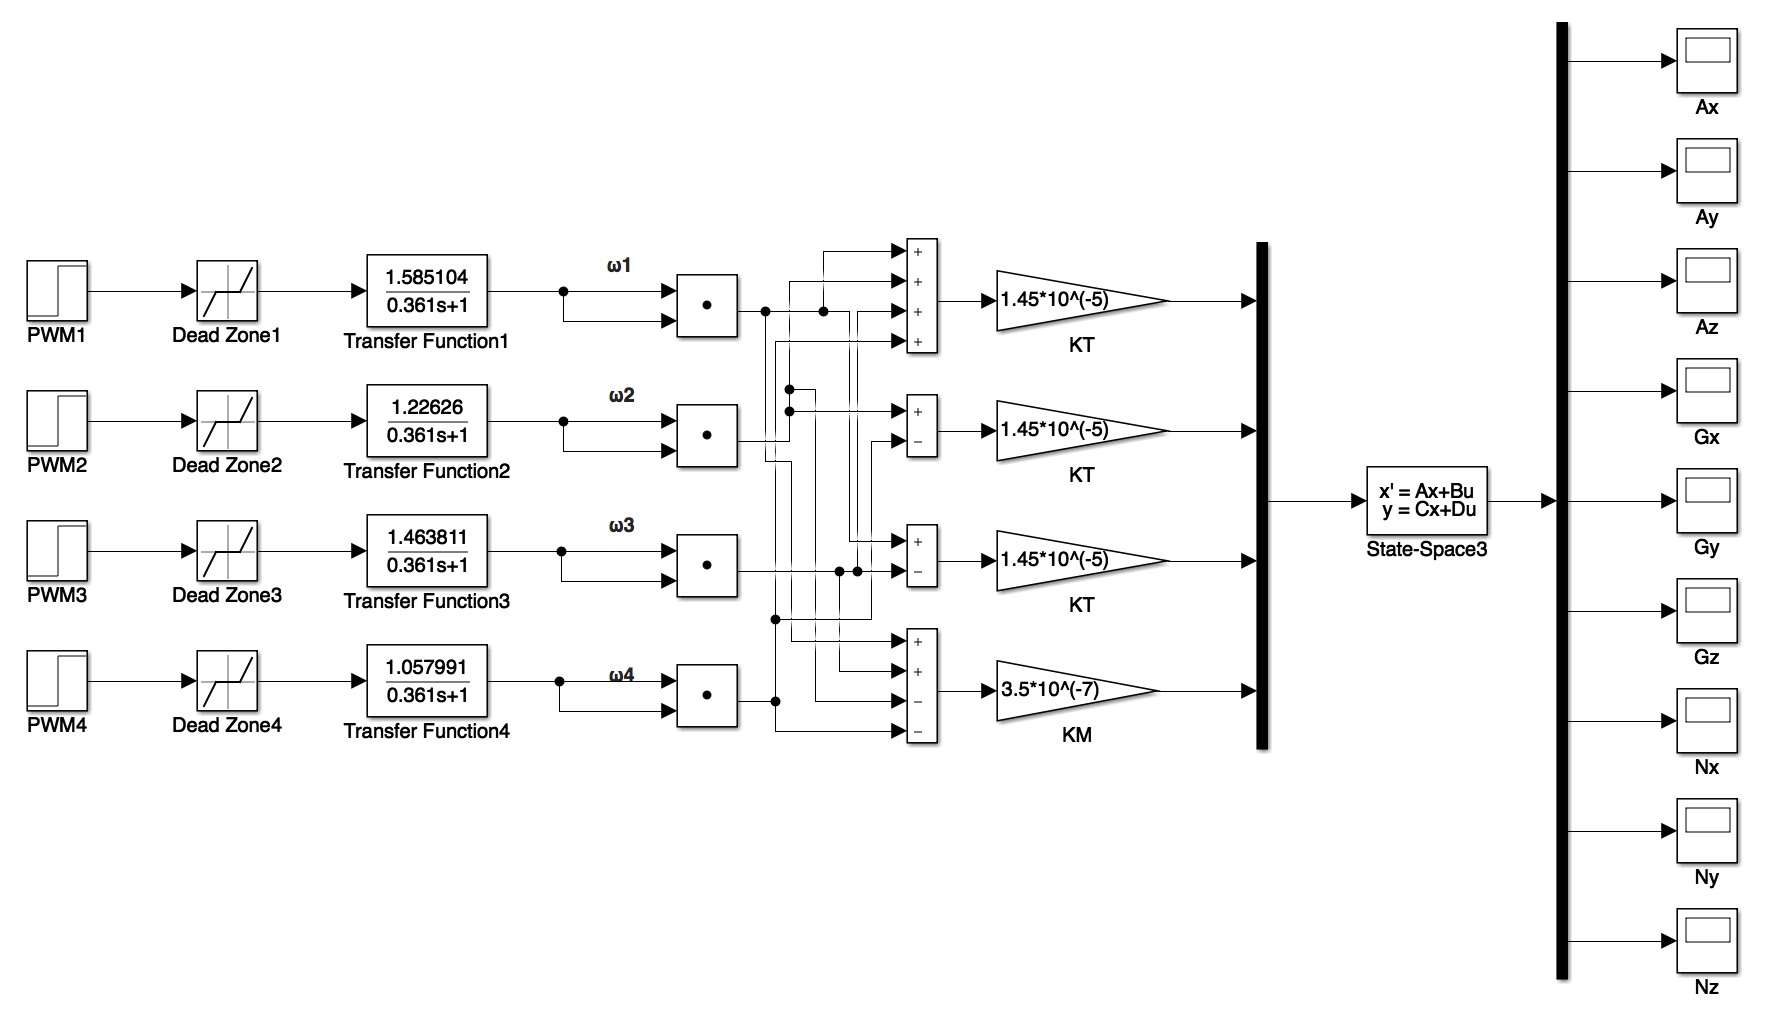
\includegraphics[width=1\textwidth]{images/openloop.png}
	\caption{Implementation of the full model.}
	\label{openloop}
\end{figure}

The response of each scope was then analysed and what was obtained is graphically shown in Figures \ref{openloop1}-\ref{openloop5}. 

\begin{figure}[H]
  \centering
    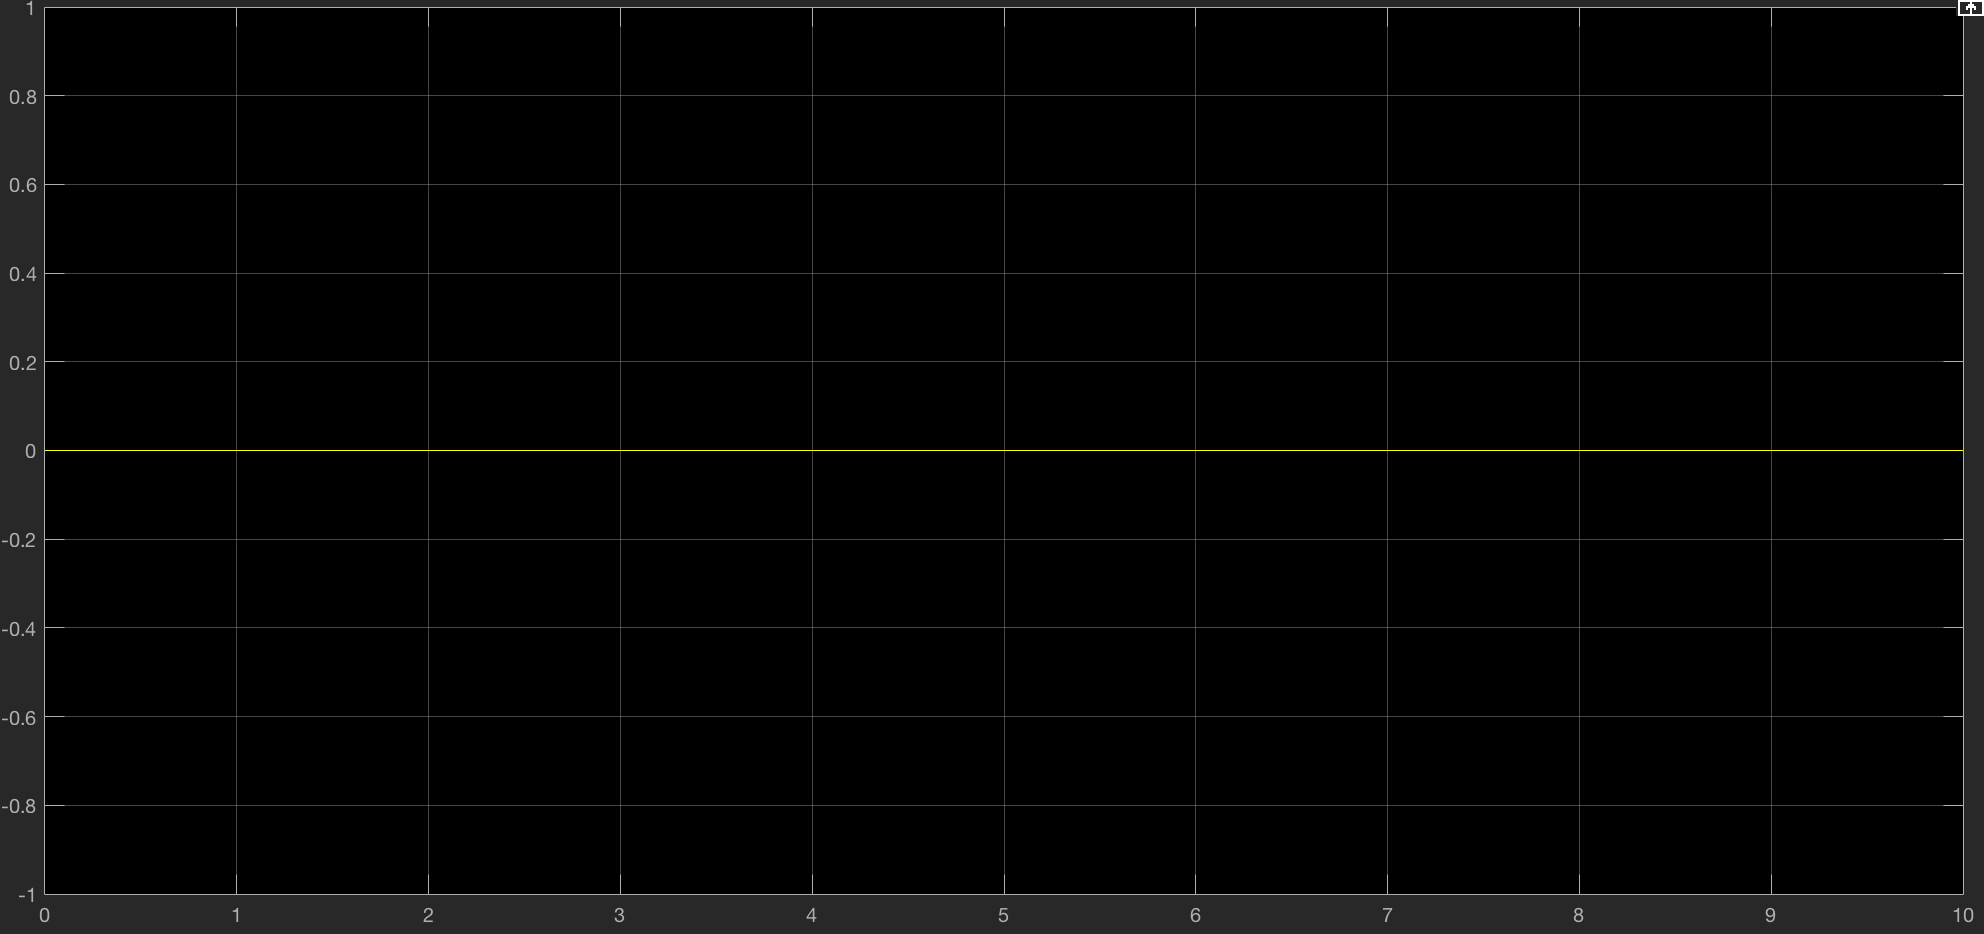
\includegraphics[width=1\textwidth]{images/Ax.png}
	\caption{Open-loop response of the Ax, Ay, Az, Nx and Nz scopes.}
	\label{openloop1}
\end{figure}

\begin{figure}[H]
  \centering
    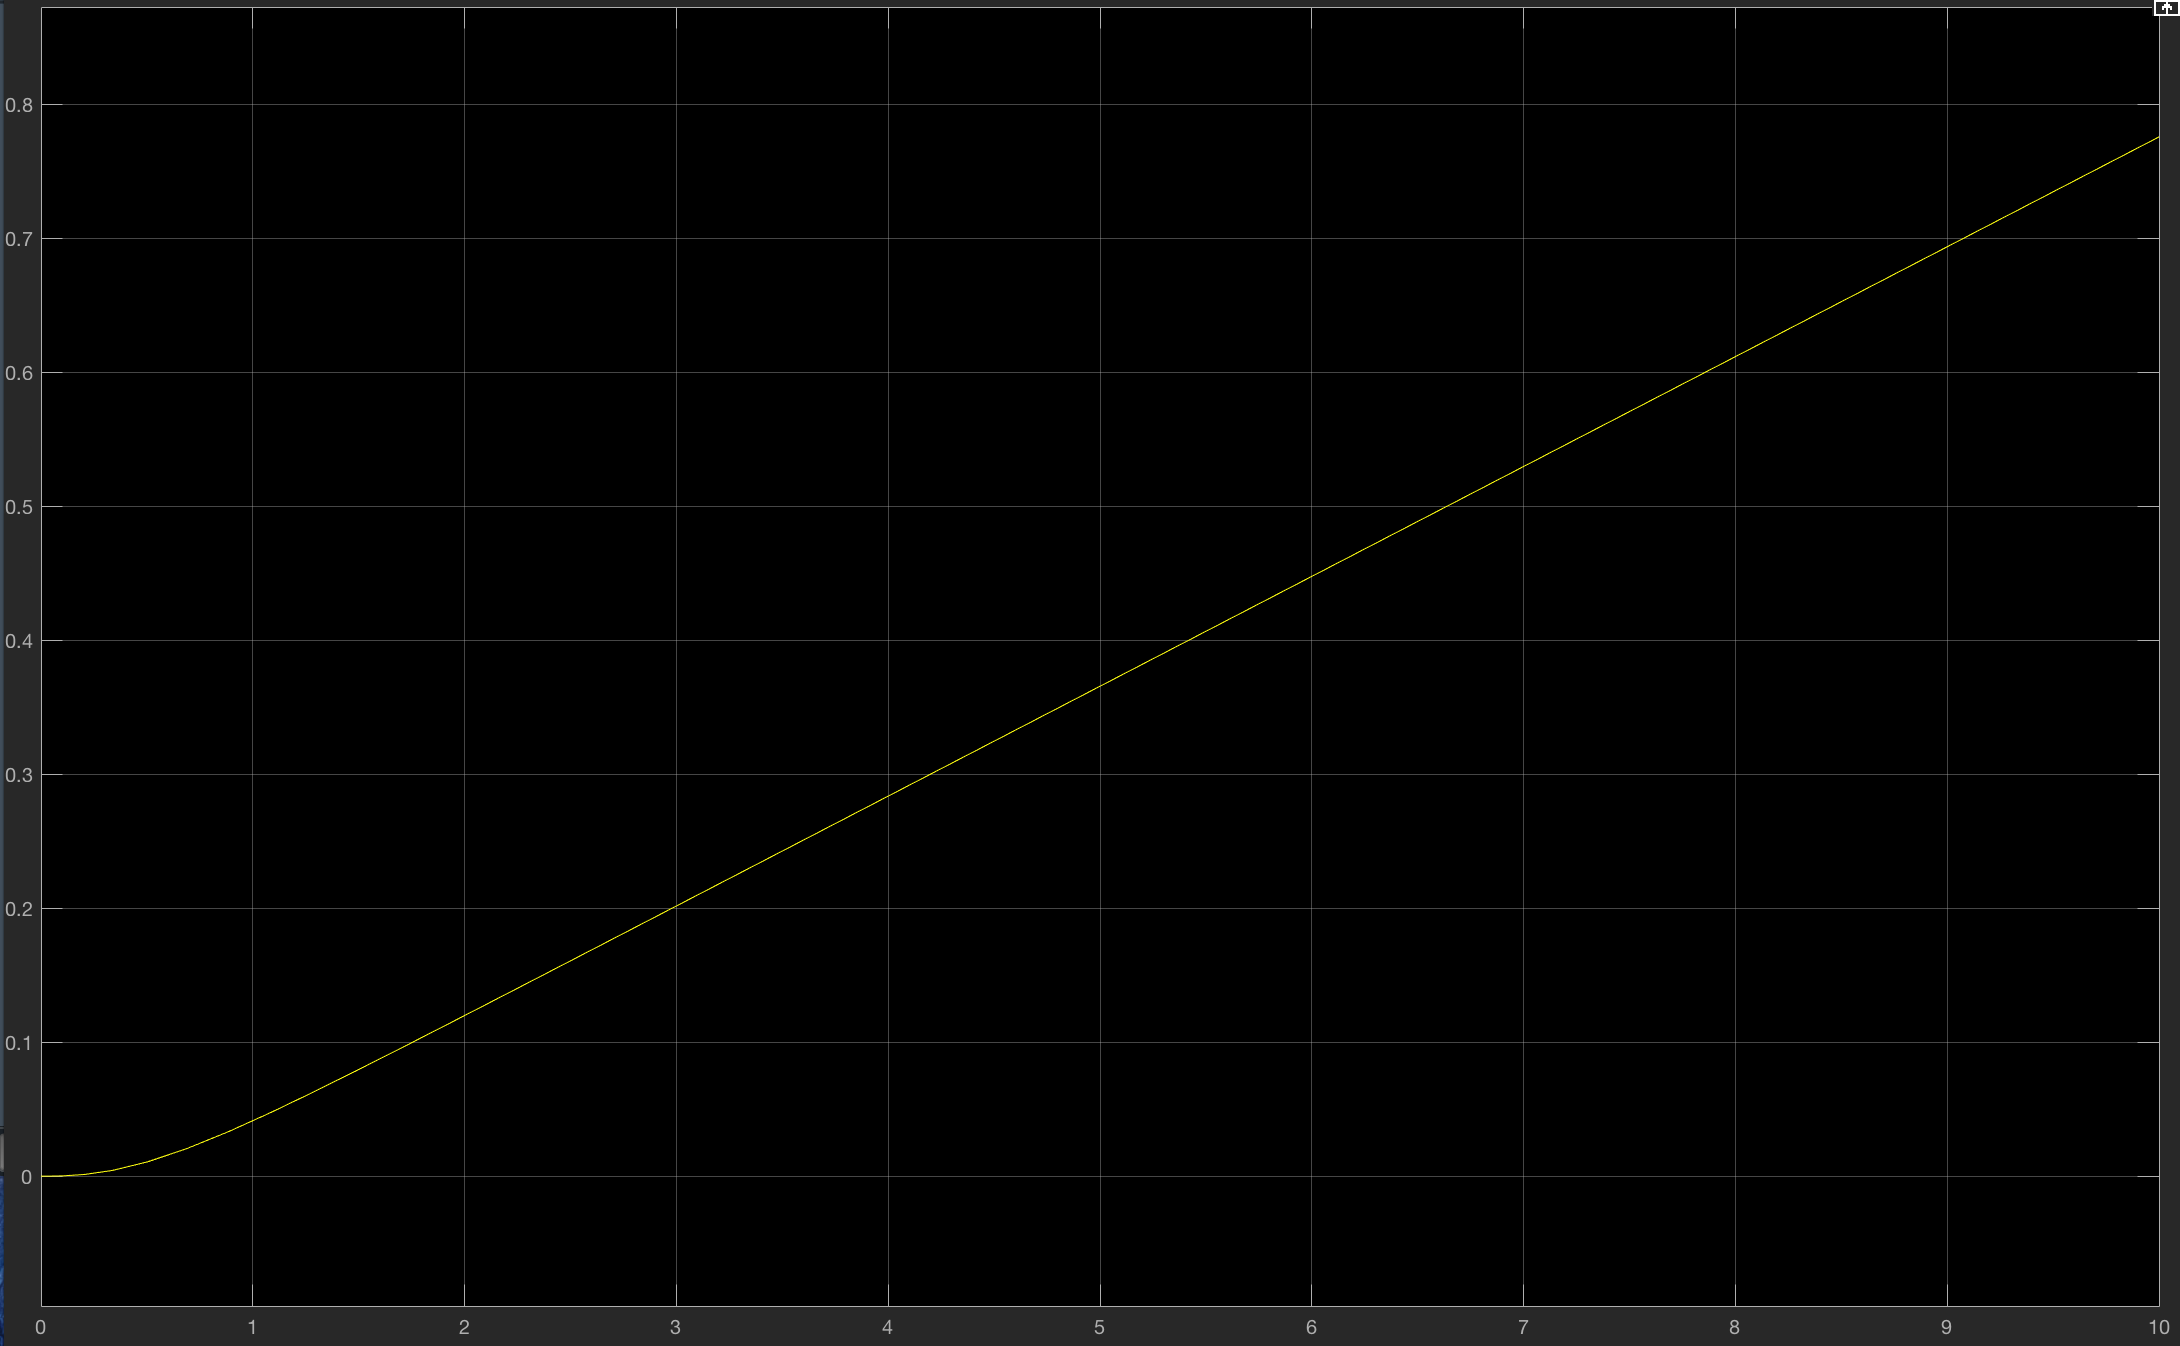
\includegraphics[width=1\textwidth]{images/Gx.png}
	\caption{Open-loop response of the Gx scope.}
	\label{openloop2}
\end{figure}

\begin{figure}[H]
  \centering
    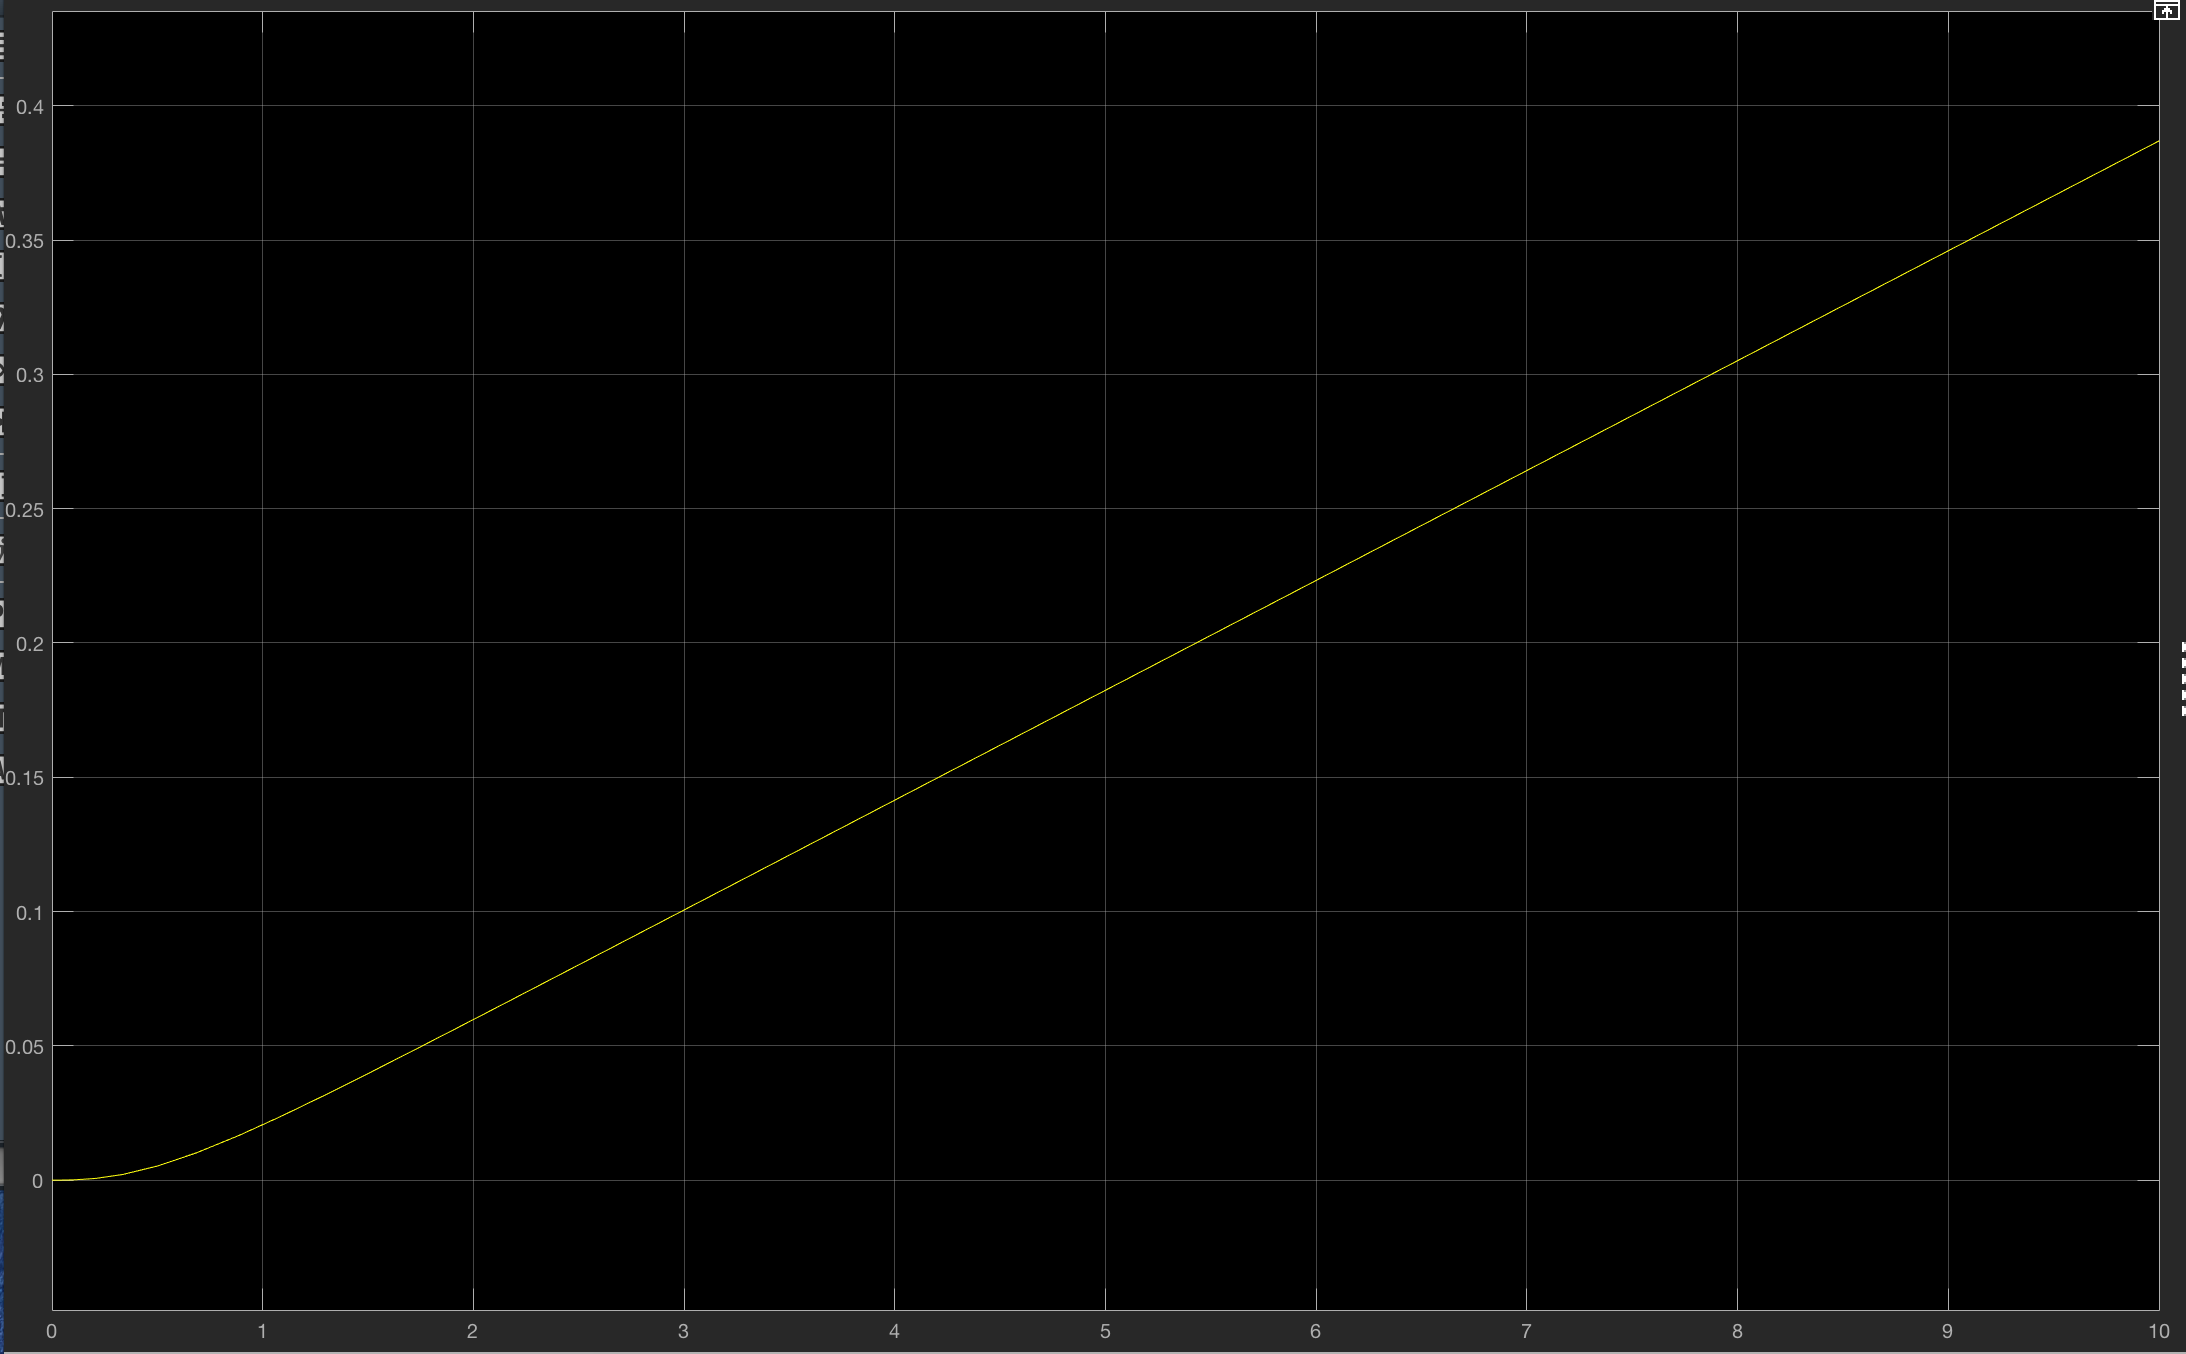
\includegraphics[width=1\textwidth]{images/Gy.png}
	\caption{Open-loop response of the Gy scope.}
	\label{openloop3}
\end{figure}

\begin{figure}[H]
  \centering
    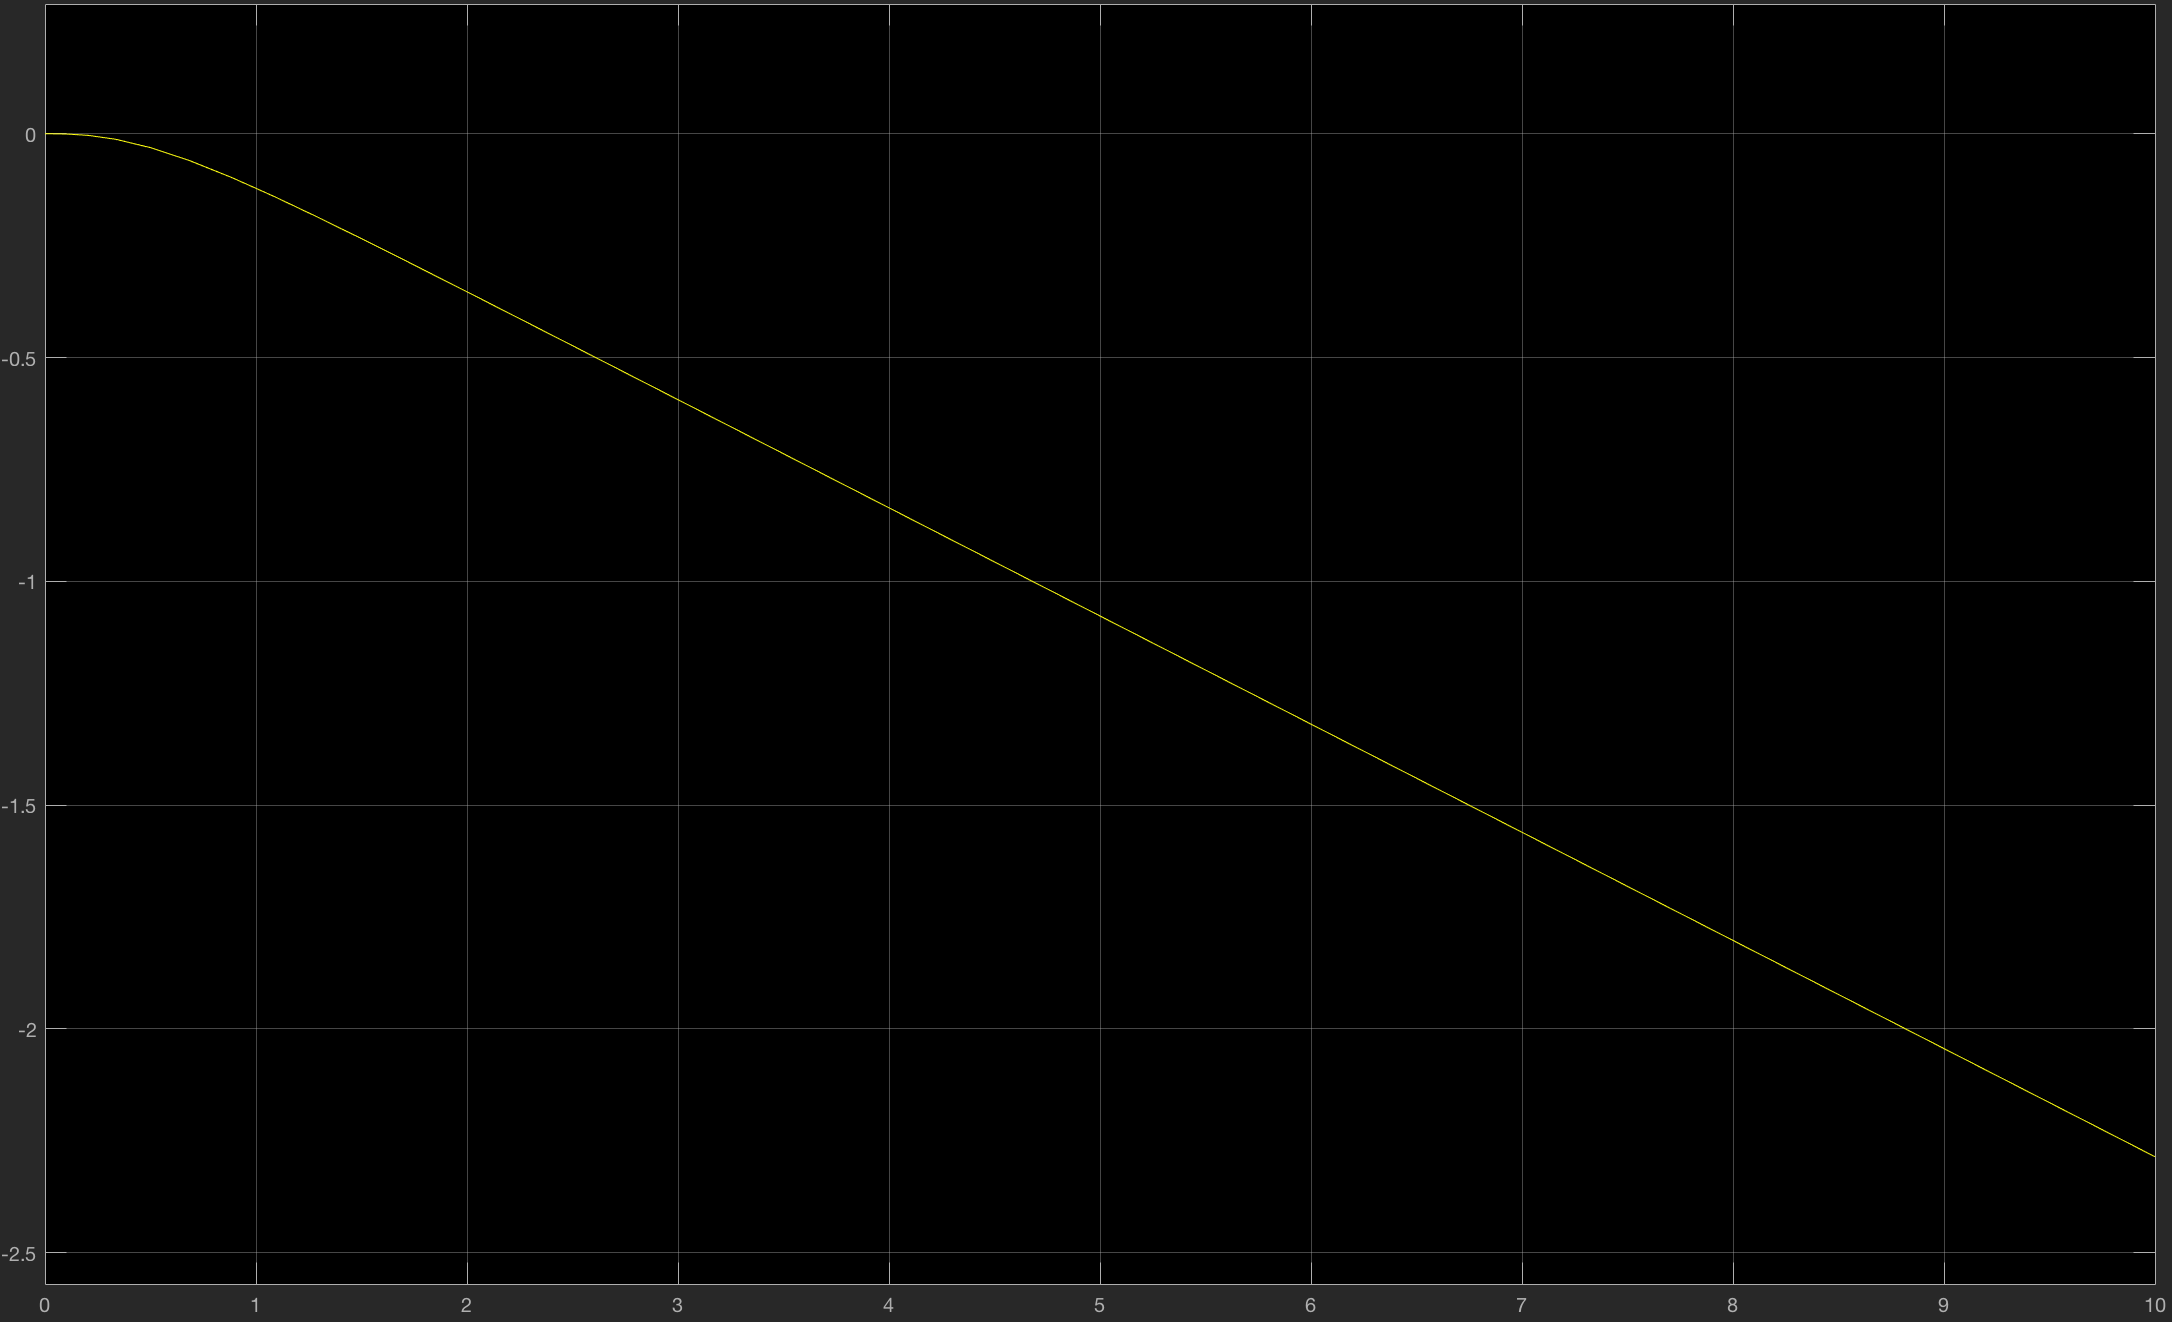
\includegraphics[width=1\textwidth]{images/Gz.png}
	\caption{Open-loop response of the Gz scope.}
	\label{openloop4}
\end{figure}

\begin{figure}[H]
  \centering
    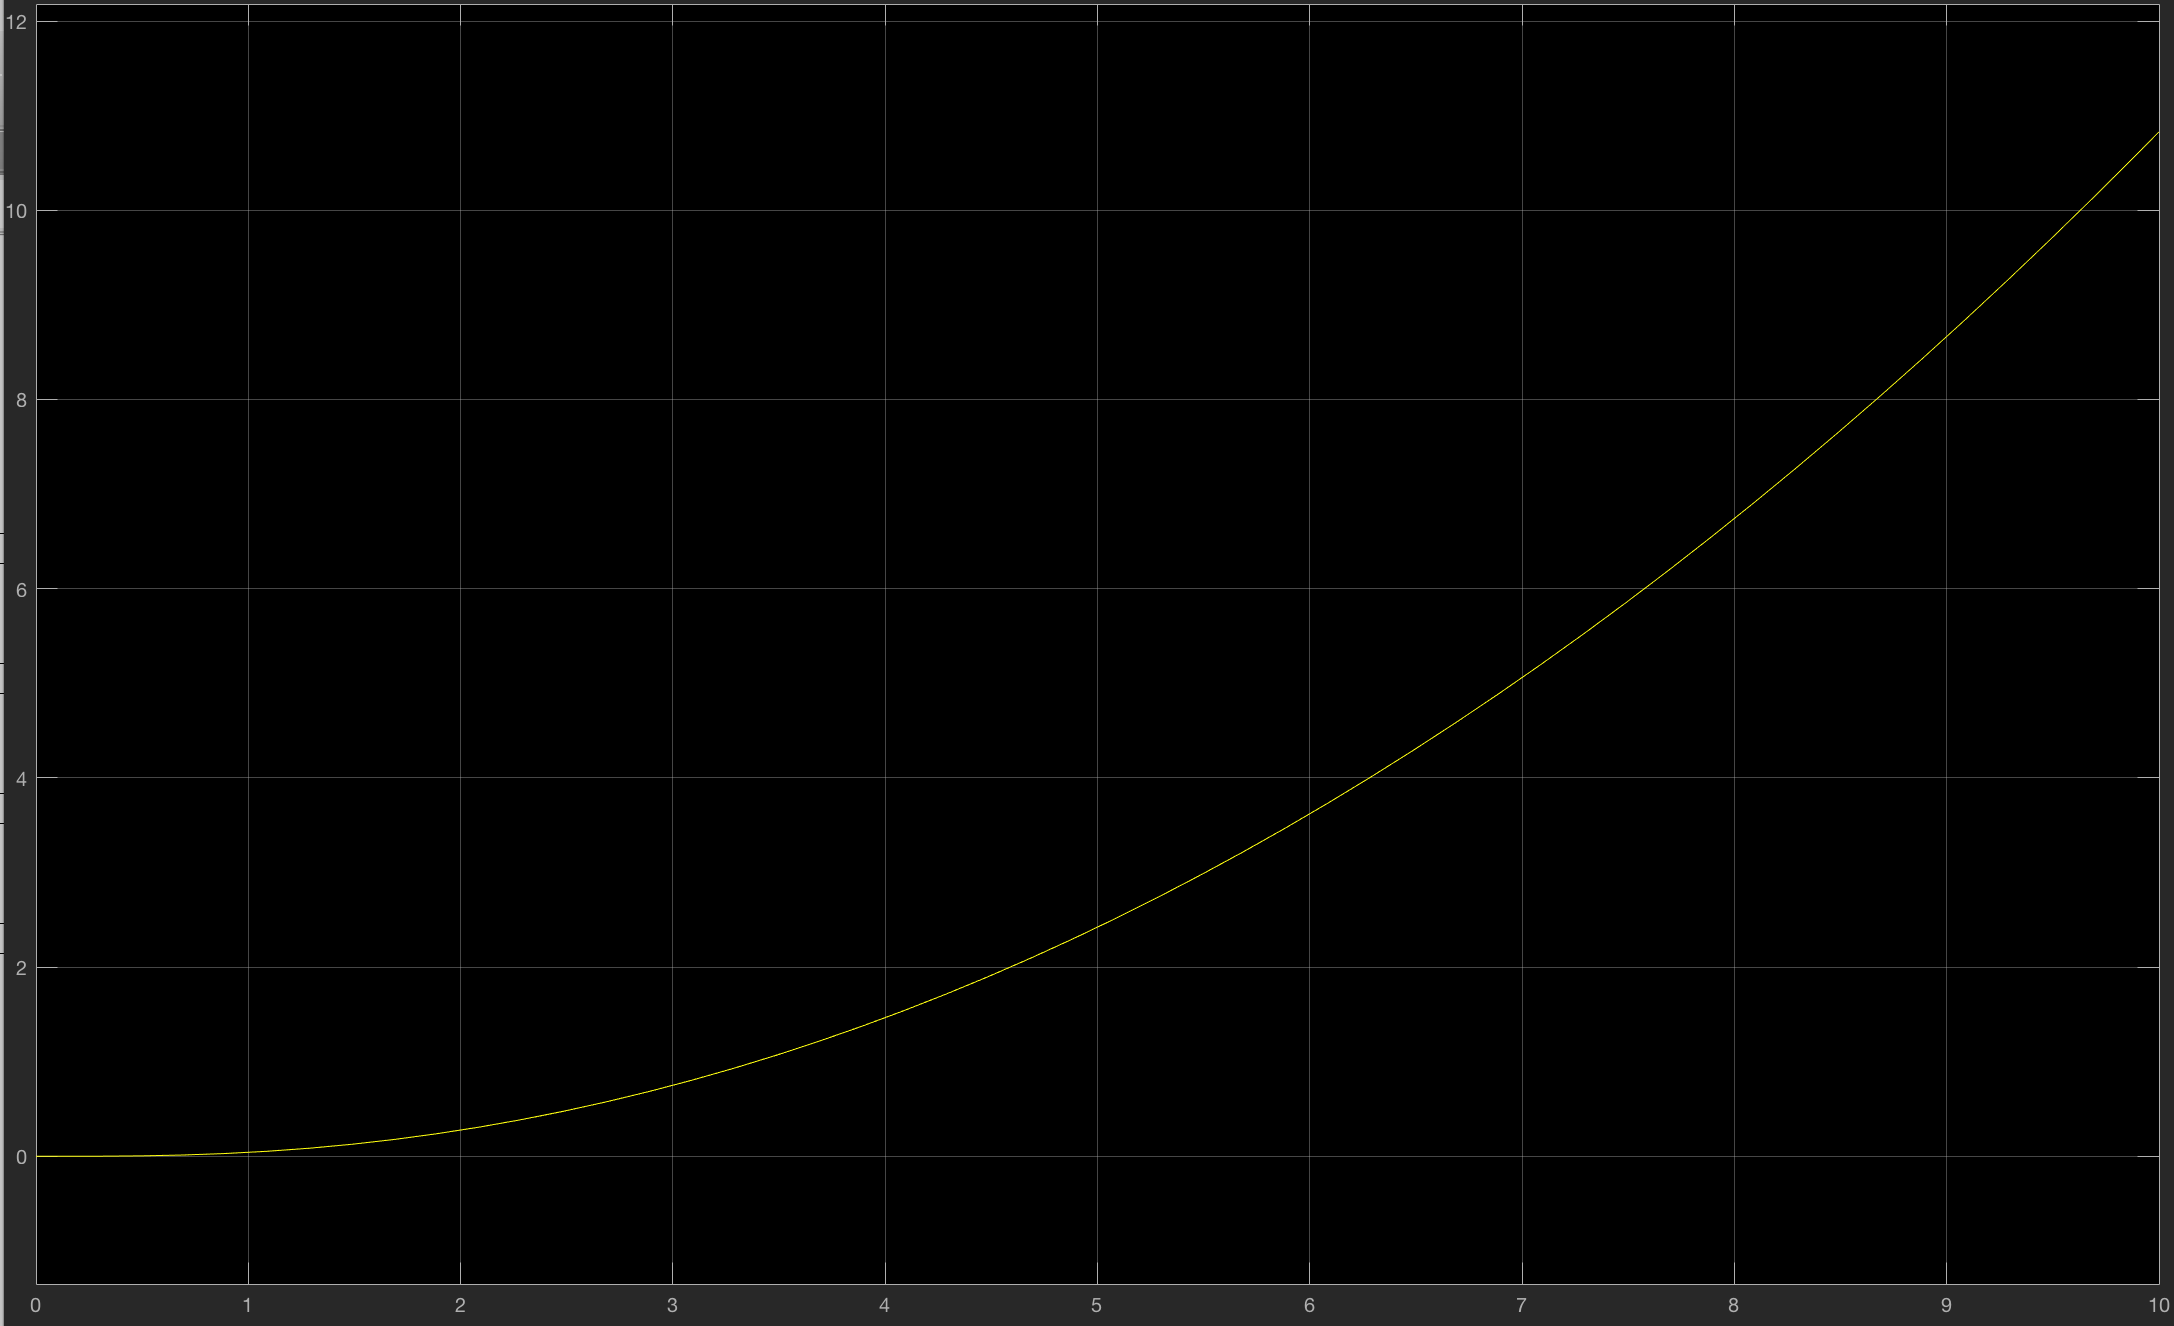
\includegraphics[width=1\textwidth]{images/Ny.png}
	\caption{Open-loop response of the Ny scope.}
	\label{openloop5}
\end{figure}

It can easily be seen that the open-loop response of the system is unstable since all the graphs look like exponentatial functions and they do not stabilise towards a desired value. This was to be expected though because, as mentioned in Section \ref{ssr}, the poles of our system are located at 0. 

This means that some kind of controller will need to be implemented in order to get the response we aim for.